\documentclass{beamer}

\usetheme{Singapore}
\setbeamercolor{alerted text}{fg=orange}
\setbeamercolor{background canvas}{bg=black}
\setbeamercolor{block body alerted}{bg=normal text.bg!90!black}
\setbeamercolor{block body}{bg=normal text.bg!90!black}
\setbeamercolor{block body example}{bg=normal text.bg!90!black}
\setbeamercolor{block title alerted}{use={normal text,alerted
text},fg=alerted text.fg!75!normal text.fg,bg=normal text.bg!75!black}
\setbeamercolor{block title}{bg=blue}
\setbeamercolor{block title example}{use={normal text,example
text},fg=example text.fg!75!normal text.fg,bg=normal text.bg!75!black}
\setbeamercolor{fine separation line}{}
\setbeamercolor{frametitle}{fg=white}
\setbeamercolor{item projected}{fg=black}
\setbeamercolor{normal text}{bg=black,fg=white}
\setbeamercolor{palette sidebar primary}{use=normal text,fg=normal
text.fg}
\setbeamercolor{palette sidebar
quaternary}{use=structure,fg=structure.fg}
\setbeamercolor{palette sidebar
secondary}{use=structure,fg=structure.fg}
\setbeamercolor{palette sidebar tertiary}{use=normal text,fg=normal
text.fg}
\setbeamercolor{section in sidebar}{fg=brown}
\setbeamercolor{section in sidebar shaded}{fg=grey}
\setbeamercolor{separation line}{}
\setbeamercolor{sidebar}{bg=red}
\setbeamercolor{sidebar}{parent=palette primary}
\setbeamercolor{structure}{bg=black, fg=black}
\setbeamercolor{subsection in sidebar}{fg=brown}
\setbeamercolor{subsection in sidebar shaded}{fg=grey}
\setbeamercolor{title}{fg=white}
\setbeamercolor{titlelike}{fg=white}

\title{Memory Efficiency and Conflict-free Replicated Data Types}
%\subtitle{Evidence from India}
\author{Ryan Bruno \and Dr. Armstrong}
\date{\today}

\begin{document}
    % Title Frame
    \begin{frame}
        \titlepage
    \end{frame}
    \begin{frame}[shrink]
        \frametitle{Problem Description}
        \begin{center}
        \begin{minipage}{4in}
          Conflict-Free Replicated Data Types (CRDTs) use extra metadata
          to allow for concurrent modifications of data without
          consensus. How can we reduce the this overhead?
        \end{minipage}
        \end{center}
    \end{frame}
    \begin{frame}[shrink]
        \frametitle{CRDT Background Information}

        \textbf{Applies to Distributed Systems with Eventual Consistency.}

        Provides Guarantees:

        \begin{enumerate}
        \item - Merge consistently.
        \item - No writes (or modifications) can be lost.
        \end{enumerate}

        OR-Set

    \end{frame}
    \begin{frame}
        \frametitle{What is Eventual Consistency?}

        CAP Theorem = Consistency, Availability, network Partitioned

        \begin{center}
        \begin{minipage}{4in}
         During a network Partition between nodes a system cannot be
         both {\color{red}Consistent} and {\color{green}Available}.
        \end{minipage}
        \end{center}
        \begin{center}
        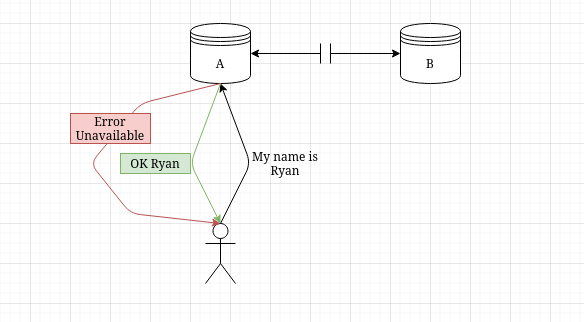
\includegraphics[width=.75\textwidth]{CapDiagram}
        \end{center}
    \end{frame}

    \begin{frame}[shrink]
        \frametitle{CRDT Background Information}

        Applies to Distributed Systems with Eventual Consistency.

        \textbf{Provides Guarantees:}

        \begin{enumerate}
            \item \textbf{- Merge consistently.}
            \item \textbf{- No writes (or modifications) can be lost.}
        \end{enumerate}

        \textbf{OR-Set}

    \end{frame}

    % PP Slides 4 - 13

    \begin{frame}
        \begin{center}
            \large{We have a problem:}
            \pause

            \large{Unbounded growth of tombstones.}
        \end{center}
    \end{frame}


    \begin{frame}[shrink]
        \frametitle{What does unbounded growth look like?}
        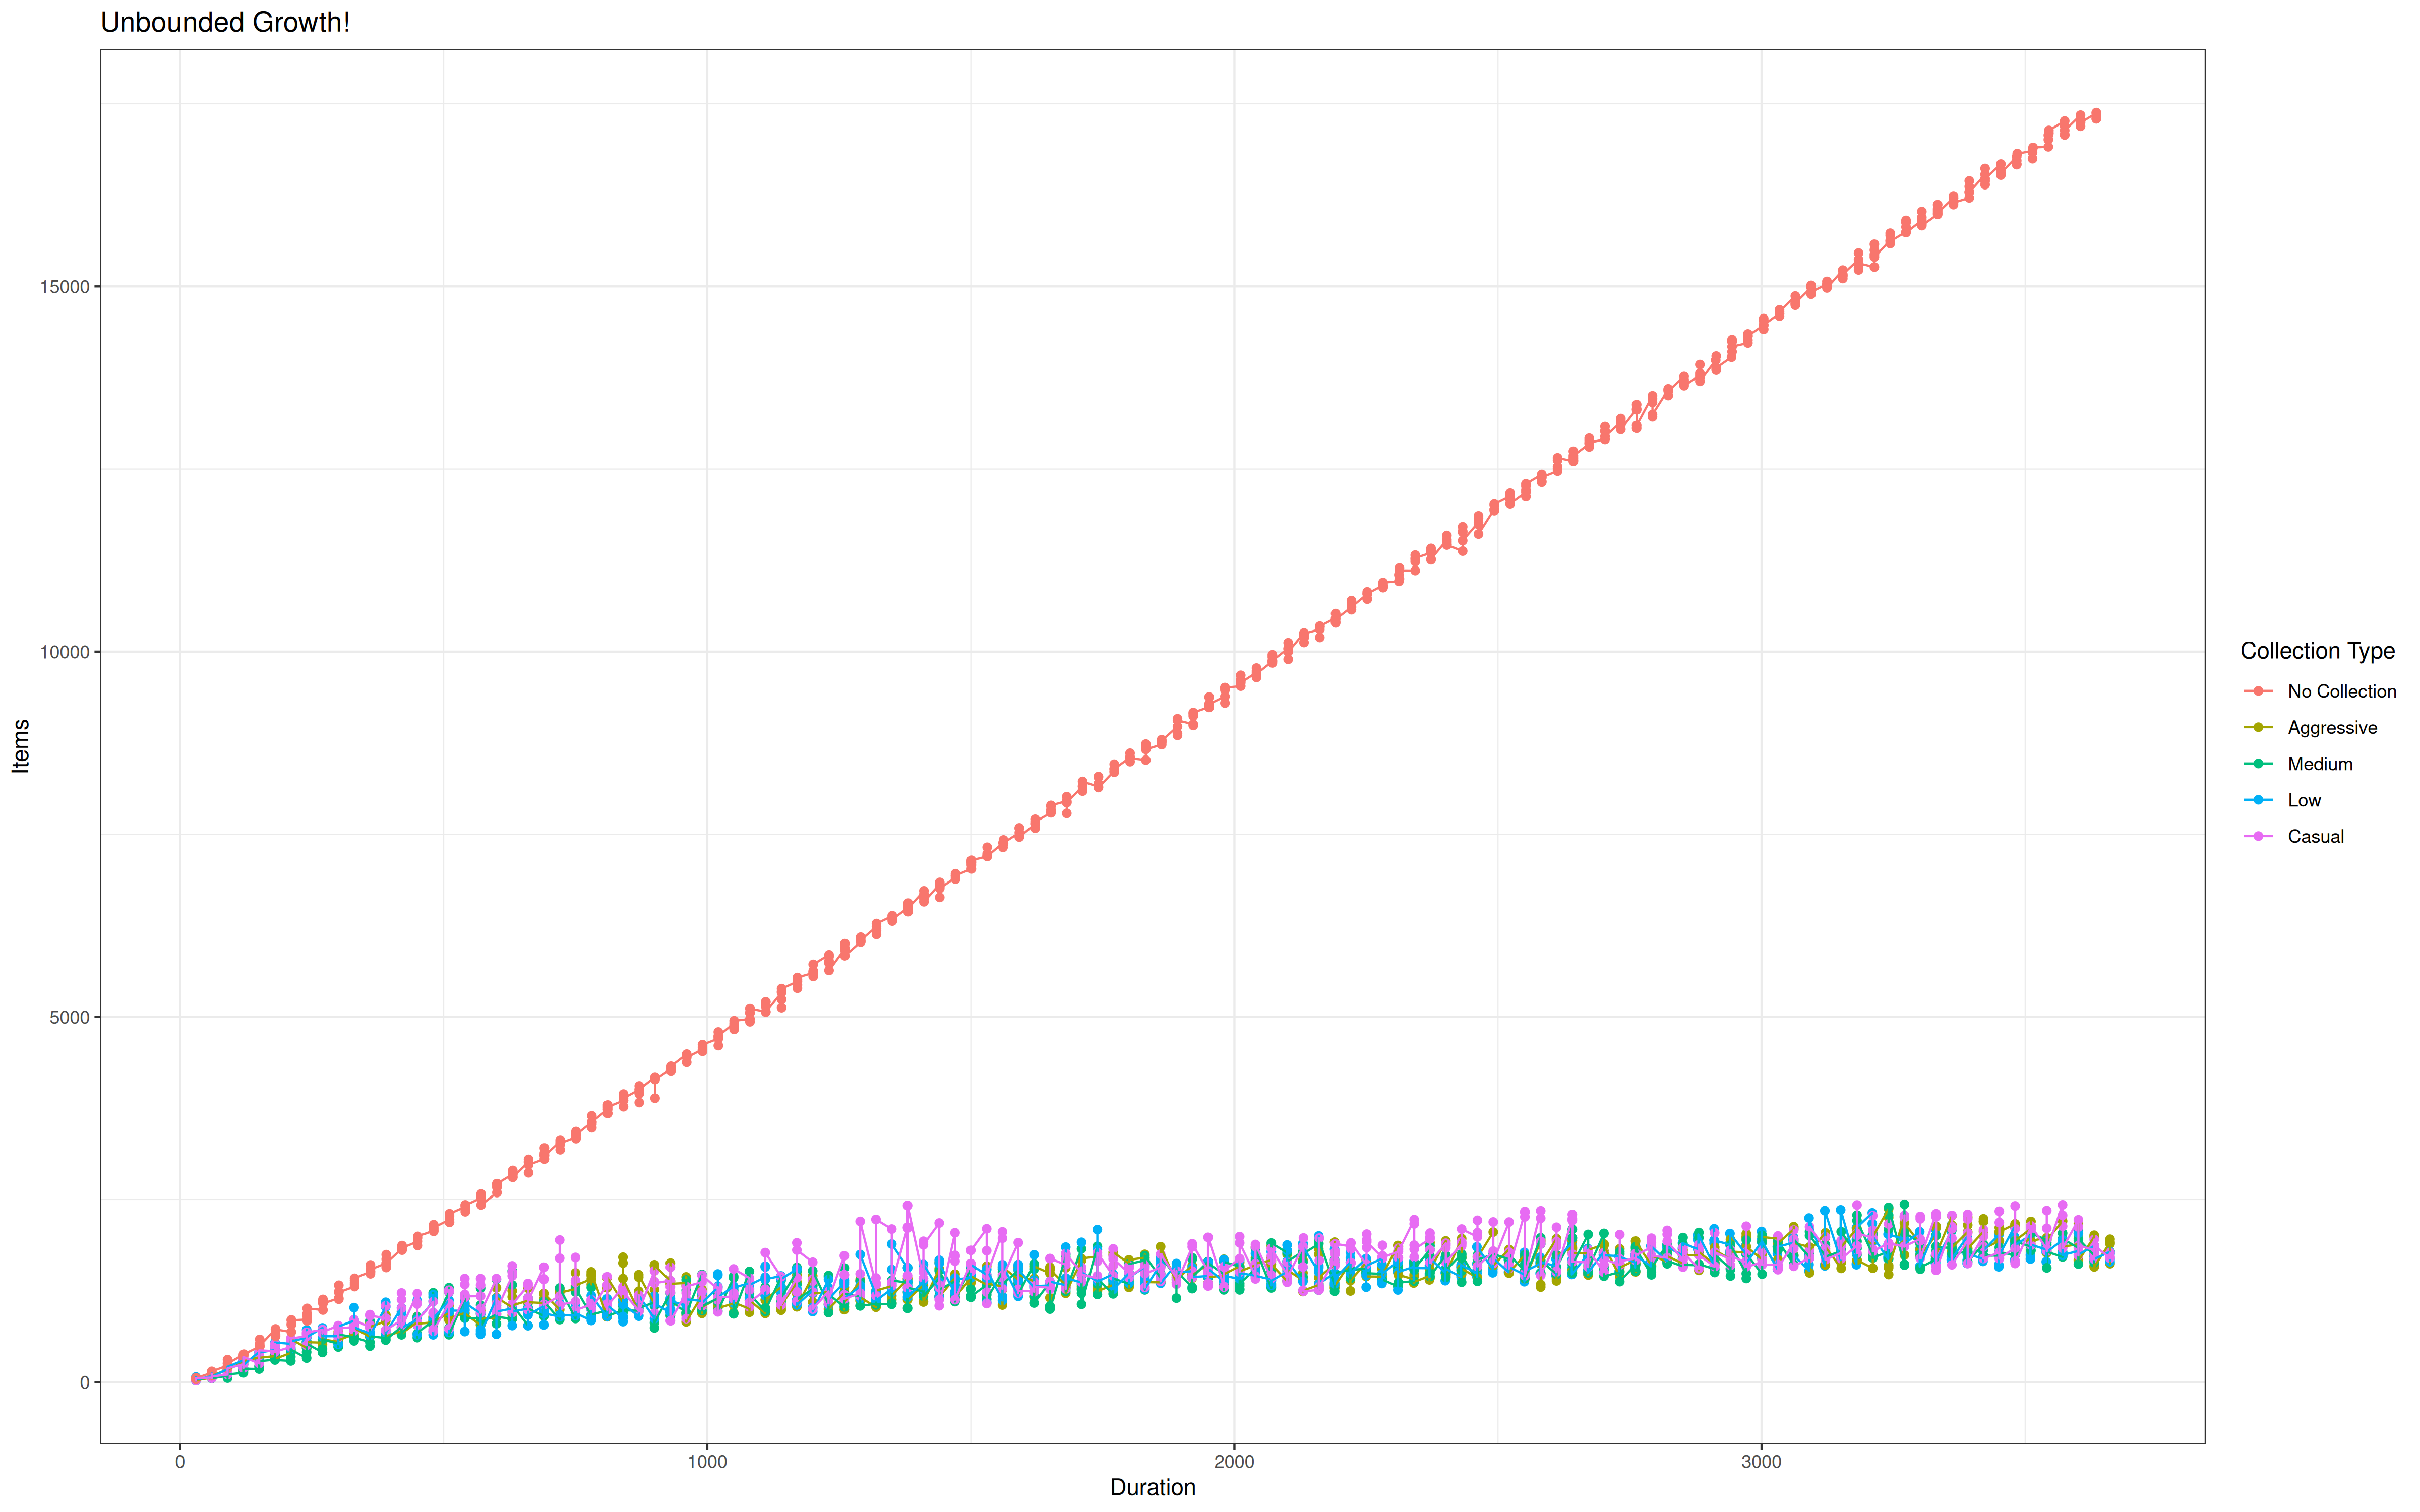
\includegraphics[width=\textwidth]{Unbounded}
    \end{frame}

    \begin{frame}
        \frametitle{Types of Collection}

        \textbf{Casual Collection}
        \begin{enumerate}
            \item \textbf{- Requires local operational ordering and bounded
                system size.}
            \item \textbf{- Implies stability.}
        \end{enumerate}

        Eager Collection
        \begin{enumerate}
            \item - Requires local operational ordering and bounded
                system size
            \item - Tracks and pushes stability.
        \end{enumerate}
    \end{frame}

    % PP Slides 15 - 16

    \begin{frame}
        \frametitle{Types of Collection}
        Casual Collection
        \begin{enumerate}
            \item - Requires local operational ordering and bounded
                system size
            \item - Implies stability.
        \end{enumerate}

        \textbf{Eager Collection}
        \begin{enumerate}
            \item \textbf{- Requires local operational ordering and bounded
                system size.}
            \item \textbf{- Tracks and pushes stability.}
        \end{enumerate}
    \end{frame}

    % PP Slides 17 - 21

    \begin{frame}[shrink]
        \frametitle{Primary Objective}
        \begin{center}
        \begin{minipage}{4in}
         To measure the memory reduction of using garbage collection in
         combination with an OR-Set while keeping the properties of a
         Conflict-free Replicated Data Type. Limited to 1.5 person
         weeks over 12 weeks.
        \end{minipage}
        \end{center}
    \end{frame}

    \begin{frame}
        \frametitle{Solution Description}
        The ORSet Research Database

        \begin{enumerate}
        \item Written in C.
        \item Communicates using RPCs.
        \item Implements Casual Collection \& Eager Collection.
        \item Configurable (1) merge rate, (2) system size, and (3) eager
            collection rate.
        \end{enumerate}
    \end{frame}

    % Results bounded growth

    \begin{frame}
        \frametitle{Results}
        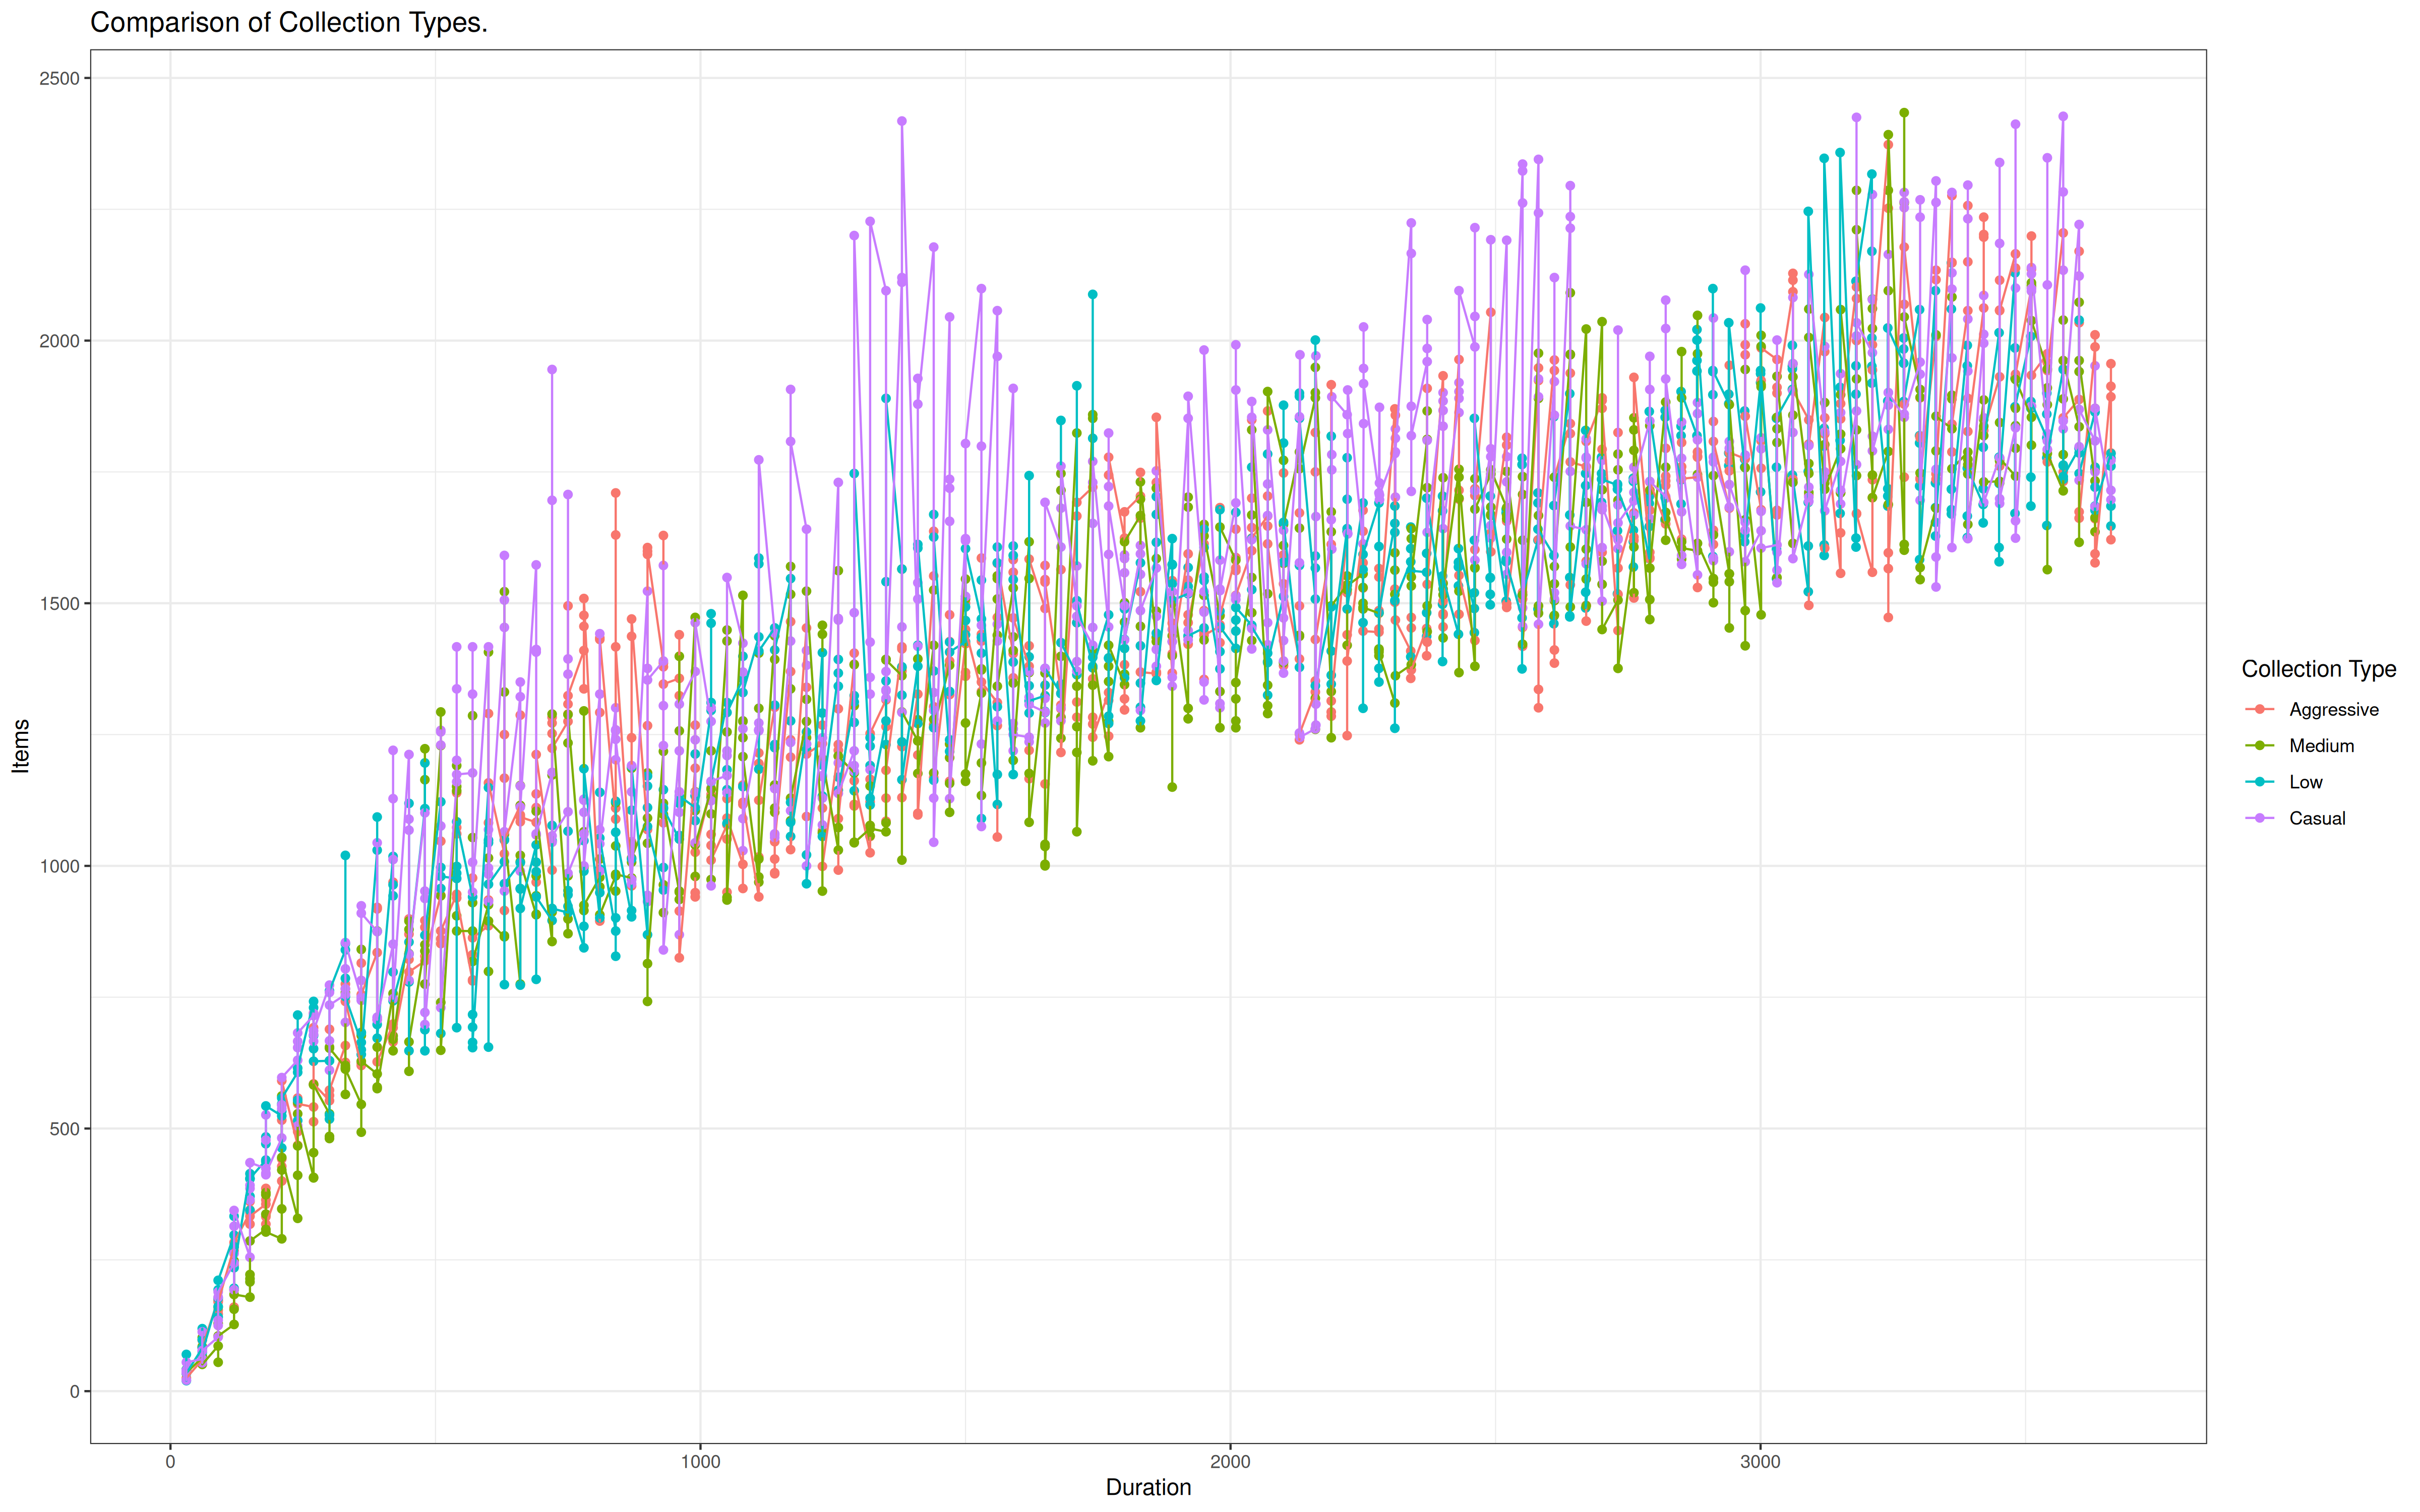
\includegraphics[width=\textwidth]{CollectionType1}
    \end{frame}
    \begin{frame}
        \frametitle{Results}
        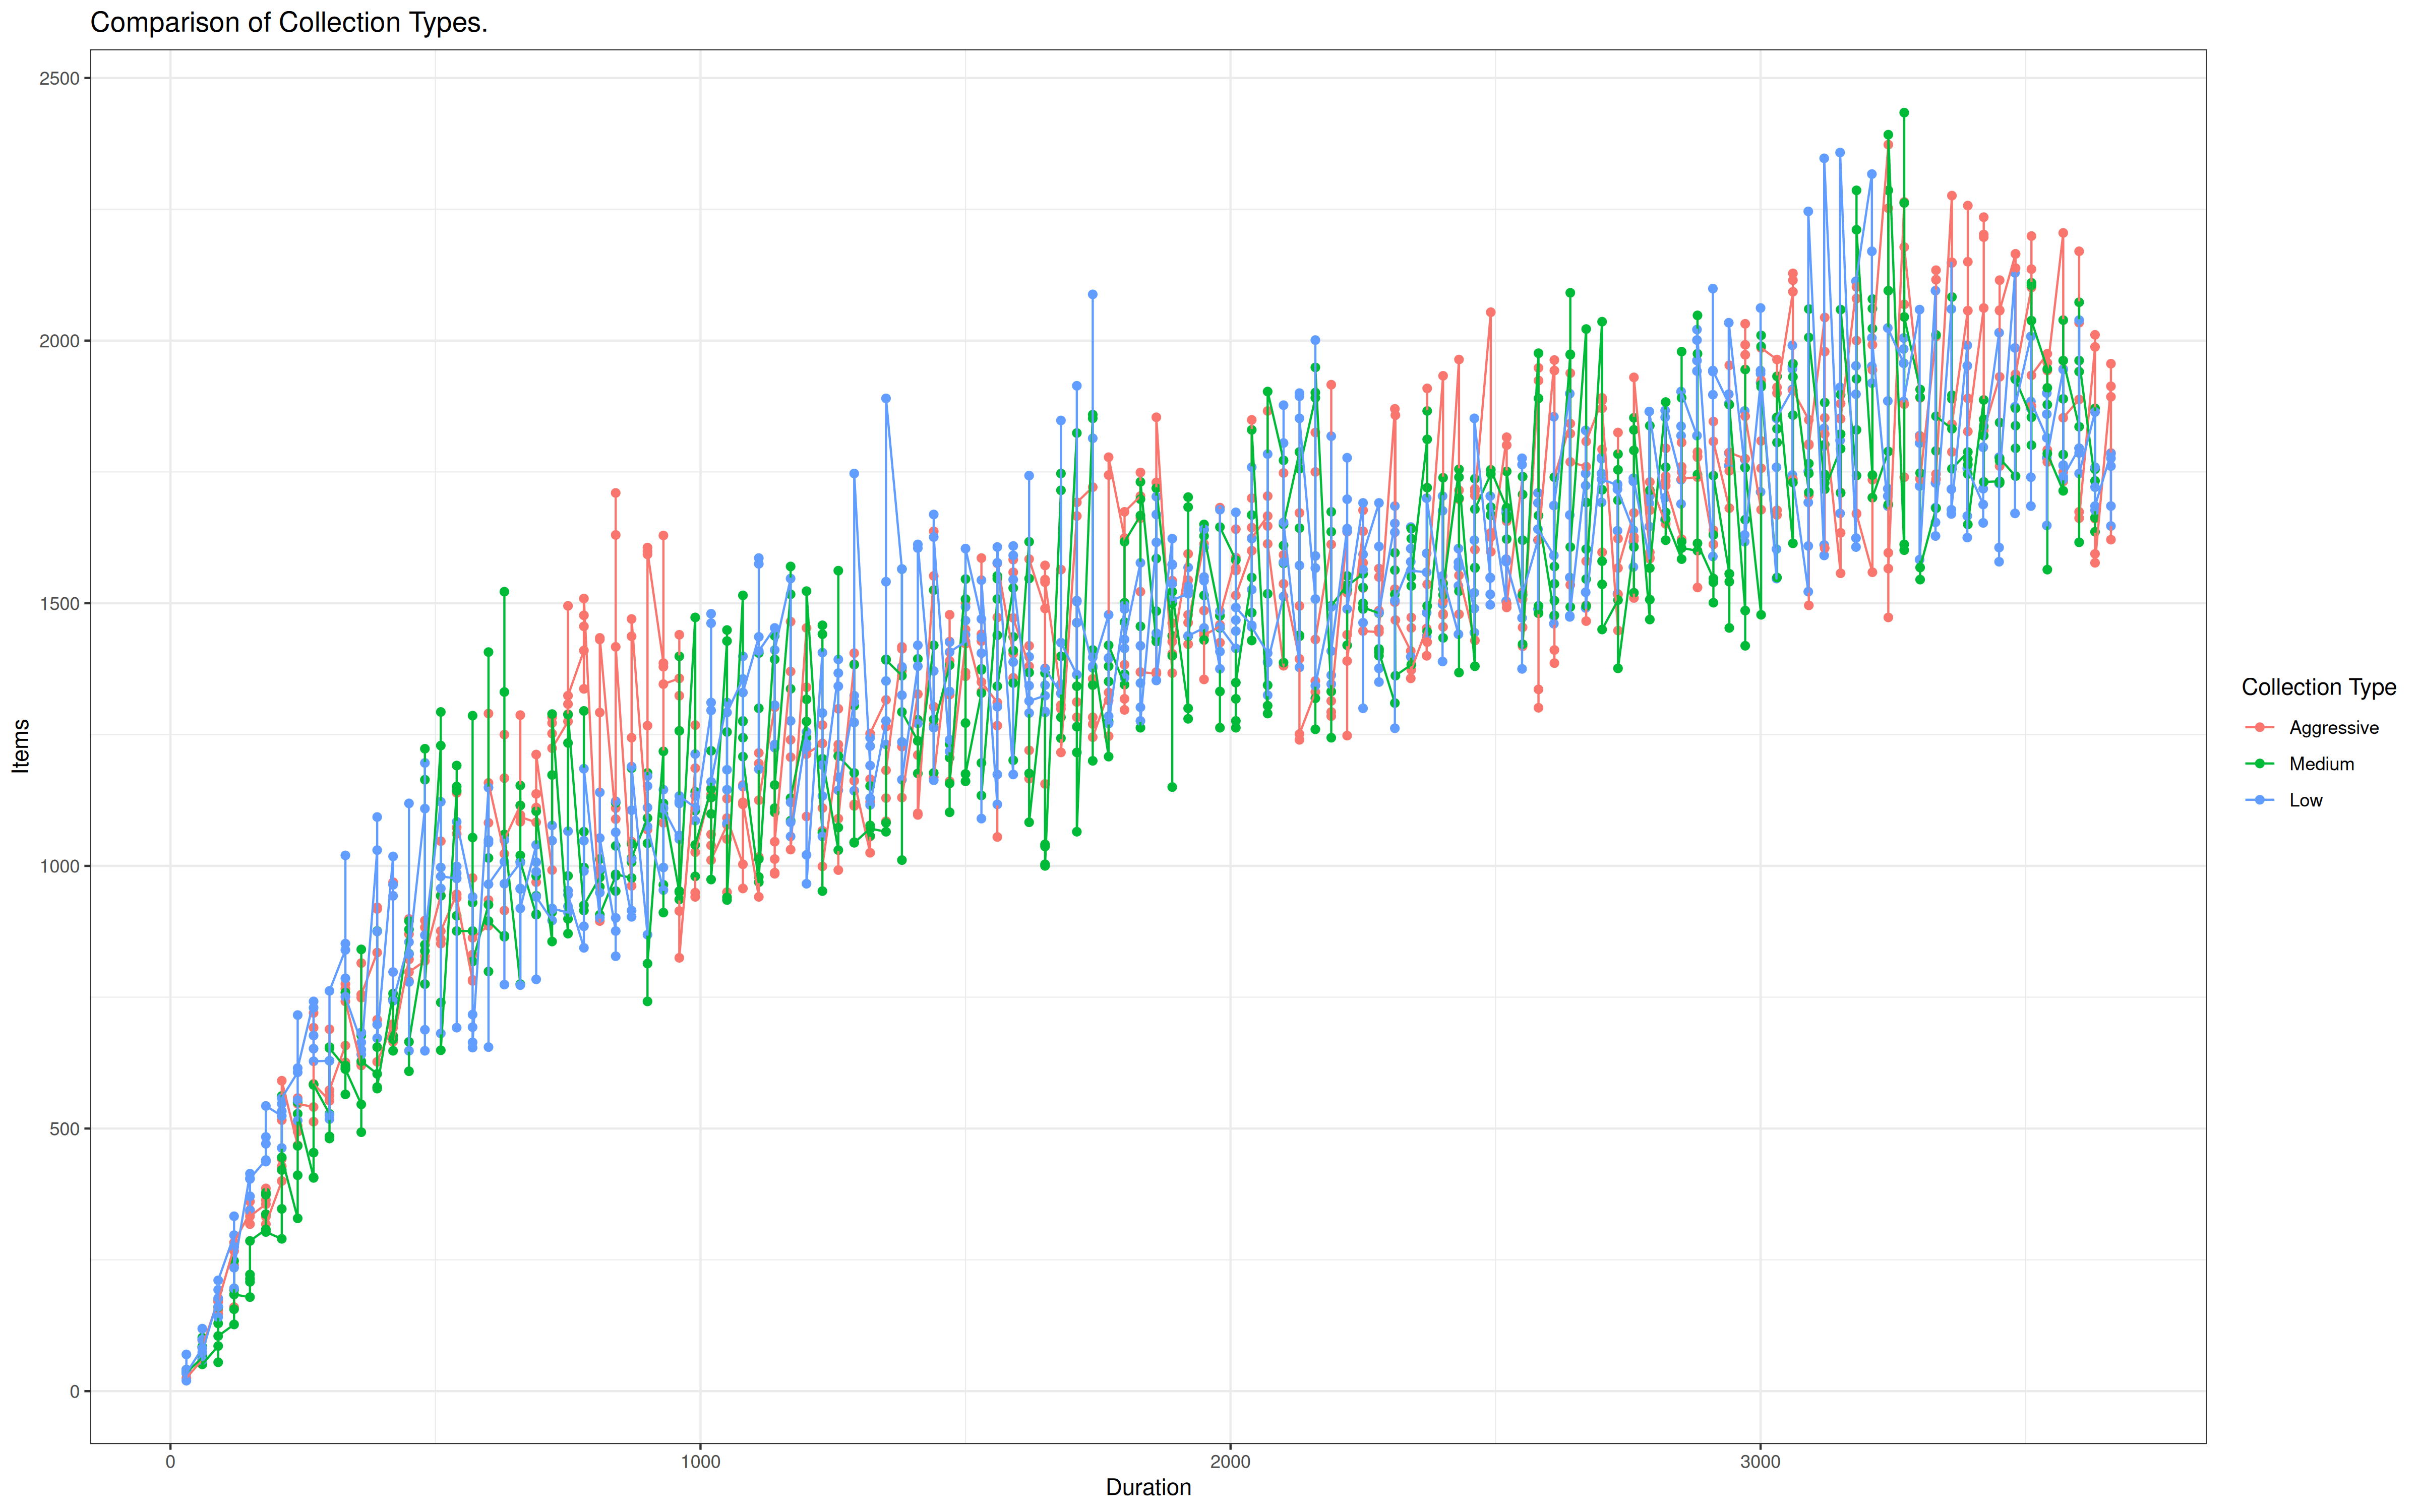
\includegraphics[width=\textwidth]{CollectionType2}
    \end{frame}

    \begin{frame}
        \frametitle{Results}
        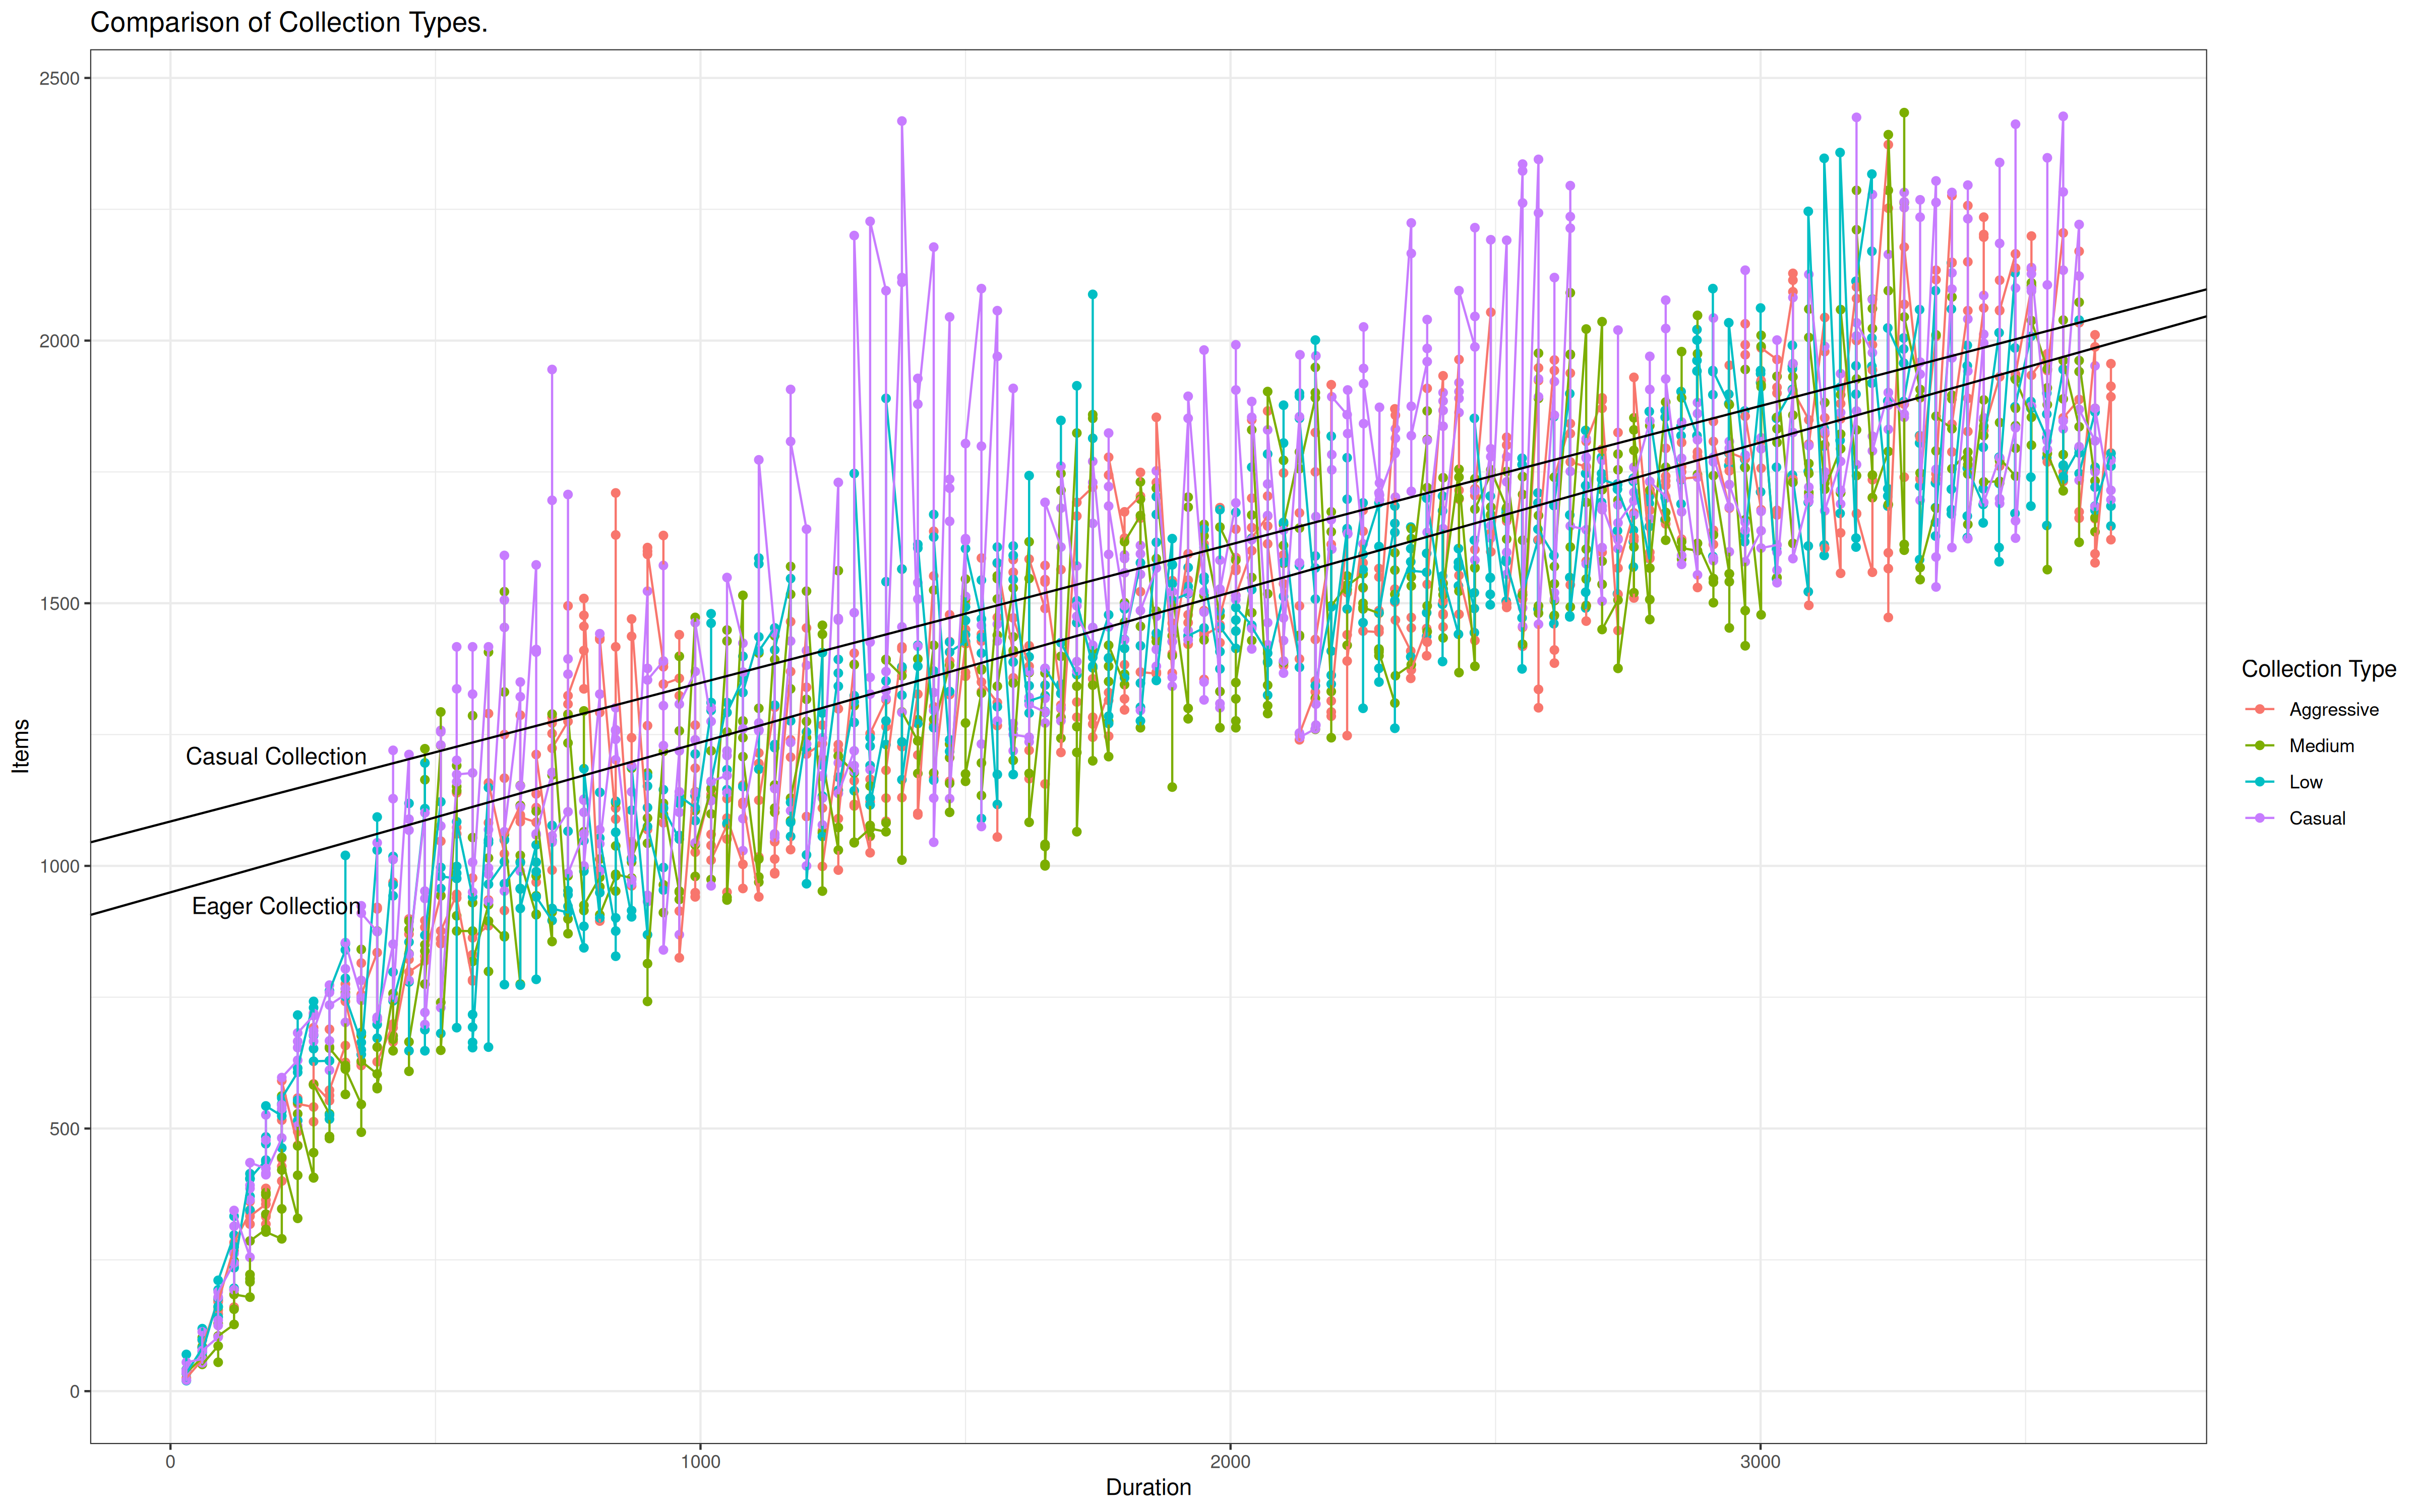
\includegraphics[width=\textwidth]{CollectionType3}
    \end{frame}

    % further research

\end{document}
